
\documentclass{package/notes}
\usepackage[english]{babel}
\usepackage{amssymb,amsmath,amsfonts}  %%% for maths
%%%%%%%%%%%%%%%%%%%%%%%%%%%%%%%%%%%%%
\usepackage{package/color-env}
\usepackage{lipsum}
\usepackage{graphicx}
\renewcommand\qedsymbol{$\blacksquare$}
\renewcommand{\bf}[1]{\textbf{#1}}
\renewcommand{\it}[1]{\textit{#1}}
%%%%%%%%%%%%%%%%%%%%%%%%%%%%%%%%%%%%%

\begin{document}

	\begin{titlepage} % Suppresses headers and footers on the title page
		
		\centering % Centre everything on the title page
		
		\scshape % Use small caps for all text on the title page
		
		\vspace*{\baselineskip} % White space at the top of the page
		
		%------------------------------------------------
		%	Title
		%------------------------------------------------
		
		\rule{\textwidth}{1.6pt}\vspace*{-\baselineskip}\vspace*{2pt} % Thick horizontal rule
		\rule{\textwidth}{0.4pt} % Thin horizontal rule
		
		\vspace{0.75\baselineskip} % Whitespace above the title
		
		{\huge MATH321: Statistics for Experamentalists\\} % Title
		
		\vspace{0.75\baselineskip} % Whitespace below the title
		
		\rule{\textwidth}{0.4pt}\vspace*{-\baselineskip}\vspace{3.2pt} % Thin horizontal rule
		\rule{\textwidth}{1.6pt} % Thick horizontal rule
		
		\vspace{2\baselineskip} % Whitespace after the title block
		
		%------------------------------------------------
		%	Subtitle
		%------------------------------------------------
		
		
		\vspace*{3\baselineskip} % Whitespace under the subtitle
		
		
		
		\vspace{0.5\baselineskip} 
		
		\vspace{0.5\baselineskip} 
		
		
		\vfill 
		
		%------------------------------------------------
		% Author
		%------------------------------------------------
		
		
		\vspace{0.3\baselineskip} 
		
		
		{\large Edited by\\  Trevor Bushnell} 
		
	\end{titlepage}
	\tableofcontents
%\newpage
\chapter{Describing Data with Graphs}
\section{Basic Statistical Definitions}

\begin{itemize}
    \item \bf{variable:} characteristic that changes/varies over time and/or for different individuals
    \item \bf{experimental unit:} the individual/object that a variable is being measured on
    \item \bf{measurement:} the result when a variable is actually measured on an experimental unit
    \item \bf{data:} a sample of measurements, which can come from a \it{population} or a \it{sample}.
    \begin{itemize}
        \item \it{population:} set of all measurements of interest
        \item \it{sample:} a subset of the measurements from the population
    \end{itemize}
\end{itemize}

\subsection{Types of Variables}

\begin{itemize}
    \item \bf{qualitative variables (categorical variables):} variables that measure a quality/characteristic
    \item \bf{quantitative variables:} variables that measure a numerical quantity
    \begin{itemize}
        \item \it{discrete variables:} variables that can only have integer values (no decimal points)
        \item \it{continuous variables:} variables that can take on any value (including decimal values)
    \end{itemize}
\end{itemize}


\section{Graphing Qualitative Variables}

\begin{itemize}
    \item We can use a \bf{data distribution} to describe \it{what values} have been measured and \it{how many} times each value has occurred. 
\end{itemize}


\chapter{Describing Data with Numerical Measures}
\begin{problem}
	LOOK AT SLIDE 2-73\\

	\begin{equation*}
		\begin{aligned}
			&\mu = 150, \sigma = 10\\	
			&\mu \pm \sigma = 150 \pm 10 = 140,160\\
			&\text{68\% of test scores will fall between 140 and 160}\\
			&\mu \pm % COME BACK LATER TO FINISH
		\end{aligned}
	\end{equation*}
\end{problem}

\begin{itemize}
	\item We can approximate $s$ (sample standard deviation) using the range
	\item $s \approx \frac{R}{4}$
	\item Note that $R$ is the range (largest - smallest)
\end{itemize}

\section{Measure of Relative Standing}

\begin{itemize}
	\item How many $\sigma$'s away from the mean does the measurement lie?
	\item We can answer this question using the \bf{z-score}
	\item $z = \frac{x - \bar{x}}{s}$, where $-3 \le z \le 3$
	\begin{itemize}
		\item If you get a z-score outside that range, then that value is an outlier
	\end{itemize}
	\item If you have a set of $n$ measurements on a variable $X$ that are arranged in order of magnitude, then the \bf{p-th percentile} is the value of $X$ that is \it{greater than $p\%$ of measurements and less than the remaining ($(100-p)\%$)}
\end{itemize}

\chapter{Probability and Probability Distributions}
\section{What Is Probability?}

\begin{itemize}
    \item probability is \it{the science of uncertainty}. When we run an experiment, we are unsure of what the outcome will be.
    \item the definition of probability is \bf{the chance of the event occurring}
    \item probability is a numerical value between 0 and 1 (inclusive) describing how likely an event is to occur - the larger the number, the more likely the event will occur.
\end{itemize}


\section{Events and the Sample Space}

\begin{itemize}
    \item \bf{experiment:} the process by which an observation is obtained
    \item a \bf{simple event} is the outcome that is observed on a single repitition of the experiment
    \begin{itemize}
        \item one and only one simple event can occur when the experiement is performed
        \item A simple event is denoted by $E$ with some subscript
        \item each simple event has some probability
    \end{itemize}

    \item \bf{sample space $S$:} the set of all simple events of an experiment
    \begin{itemize}
        \item \it{discrete sample space:} a sample space that contains a finite or countable infinite number of elements
        \item \it{continuous sample space:} a sample space that contains all or a subset of all real numbers
    \end{itemize}

    \item \bf{event:} a collection of one or more simple events (aka a subset of the sample space)
    \begin{itemize}
        \item EX: If the values on a 6-sided die are our sample space, then an example event would be getting an odd number
    \end{itemize}

    \item \bf{mutually exclusive:} a way to describe two events where if one event occurs, the other event cannot occur (same goes in reverse order)
\end{itemize}


\section{Set Theory Review}

\begin{itemize}
    \item Since events are just sets, we can compare relations between events by talking about relations between sets (aka using set theory)
    \item \bf{union $A \cup B$:} the event that occurs when either $A$ or $B$ occur
    \begin{itemize}
        \item $A \cup B = \{x : x \in A $ OR $x \in B\}$
    \end{itemize}
    \item \bf{intersection $A \cap B$:} the event that occurs when both $A$ and $B$ occur
    \begin{itemize}
        \item $A \cap B = \{x : x \in A $ AND $x \in B\}$
    \end{itemize}
    \item \bf{complement $A^C$ or $A'$ or $\bar A$:} means that we care about all the elements in the sample space that are NOT also in $A$. 
    \begin{itemize}
        \item $A^C = \{x : x \notin A\}$
    \end{itemize}
\end{itemize}

\begin{definition}[The Axioms of Probability]{def3.1:label}
    \begin{enumerate}
        \item For any event $A$, $P(A) \ge 0$
        \item $P(S) = 1$
        \item If $A_1, A_2, A_3, \cdots$ is a finite or countably infinite sequence of mutually exclusive events of $S$, then $P(A_1 \cup A_2 \cup A_3) = P(A_1)+P(A_2)+P(A_3)$
    \end{enumerate}
\end{definition}

Using the axioms above, then you can come up with these theorems:

\begin{theorem}[Consequences of the Axioms of Probability]{th3.1:label}
    \begin{enumerate}
        \item If $A$ and $A^C$ are complementary events in a sample space $S$, then $P(A^C) = 1 - P(A)$
        \item $P(\varnothing) = 0$ for any sample space $S$
        \item If $A$ and $B$ are events in a sample space $S$ and $A \subset B$, then $P(A) \le P(B)$
        \item If $A$ and $B$ are any two events in a sample space $S$, then $P(A \cup B) = P(A) + P(B) - P(A \cap B)$
    \end{enumerate}
\end{theorem}


\section{Calculate Probabilities Using Simple Events}

\begin{definition}[Probability of a Simple Event]{def3.2:label}
    The probability of event $A$ is equal to 

    $$
    \frac{n}{N}
    $$

    where $n = |A|$ and $N = |S|$. In other words, the probability of a simple event is equal to the number of possible outcomes for the desired event divided by the total number of outcomes
\end{definition}

\chapter{Random Variables}
\section{Definition of Random Variables}

\begin{itemize}
    \item If we have an experiment with a sample space $S$, then a \bf{random variable} $X$ is a set function that assigns unique real numbers $X(s)=x$ to each element $s \in S$
    \begin{itemize}
        \item IN OTHER WORDS: This variable $X$ takes on some value based on the random outcome from the experiment
    \end{itemize}

    \item The \bf{space} of $X$ is the set of all real numbers: $\{x:X(s) = x, s \in S\}$
    \item We typically represent random variables with capital letters while the lowercase letters are your typical variables that you encounter in algebra/calculus that can take on any possible value
\end{itemize}


\section{Discrete VS Continuous Random Variables}

\begin{itemize}
    \item \bf{discrete random variables:} random variables whose set of possible values is either finite or countably finite (can only take on whole number values)
    \item \bf{continuous random variables:} random variables whose set of values is uncountable (can take on whole value and decimal values)
\end{itemize}


\section{Probability Functions}

\begin{definition}[Probability Mass Function (pmf)]{def4.1:label}
    The \bf{probability mass function} is a function that describes a \it{discrete random variable} that satisfies the following properties:

    \begin{enumerate}
        \item $P(X = x) = f(x) > 0$ if $x \in S$
        \item $\sum_{x \in S} f(x) = 1$
        \item $P(A) = \sum_{x \in A} f(x)$ where $A \in S$
    \end{enumerate}
\end{definition}

\begin{definition}[Cumulative Distribution]{def4.2:label}
    If $X$ is a discrete random variable, then the function given by:

    $$
    F(x) = P(X \le x) = \sum_{t \le x} f(t)
    $$

    for $-\infty < x < \infty$ is called the \bf{cumulative distribution function (cdf)}. The cumulative distribution satisfies the following properties:

    \begin{enumerate}
        \item $F(-\infty) = 0$ and $F(\infty) = 1$
        \item if $a < b$, then $F(a) \le F(b)$ for any real numbers $a$ and $b$
    \end{enumerate}

    \begin{itemize}
        \item Random variables are defined in terms of functions which in turn must have distributions.
        \item This means that we can find the mean and the standard deviation
        \item the \it{mean} is also called the \bf{expected value} and is calculated using $\mu = E(x) = \sum xf(x)$
        \item the \it{variance} is calculated using: $\sigma = \sum (x-\mu)^2f(x)$
        \item you can also calculate variance using: $\sigma^2 =E(X)^2 - [E(X)]^2$
        \item The \it{standard deviation} can be calculated using $\sigma = \sqrt{\sigma^2}$
    \end{itemize}
\end{definition}


\chapter{Several Useful Discrete Distributions}
\section{Introduction}

\begin{itemize}
    \item Discrete random variables take on only a finite or countable infinite number of values
    \item There are three discrete probability distributions which will serve as modes for a large number of stats models/applications, which are as follows:
    \begin{enumerate}
        \item \bf{binomial} distribution
        \item \bf{poisson} distribution
        \item \bf{hypergeometric} distribution
    \end{enumerate}
\end{itemize}

\section{Binomial Distribution}

\begin{itemize}
    \item Bernoulli trial is an experiment with only two possible outcomes (success and failure)
    \item These have probabilities $p$ and $1-p$
    \item A coin tossing experiment is an example that uses this distribution 
\end{itemize}

\subsection{The Binomial Experiment}

\begin{enumerate}
    \item Consists of $n$ identical trials
    \item Each trial has one of two outcomes, success or failure
    \item The probability for each trial remains constant
    \item the trials are independent
    \item We are interested in $X$, the number of successes in $n$ trials
\end{enumerate}\newpage

\begin{definition}[The Binomial Prbability Distribution]{def5.1:label}
    For a binomial experiment that has $n$ trials and probability $p$ of a success, then the probability of $k$ successes in $n$ trials is:

    $$
    P(X = k) = \binom{n}{k}p^kq^{n-k} \text{ for } 0 \le k \le n
    $$
\end{definition}

Here are some formulas for the basic stats of the Binomial Bistribution:

\begin{itemize}
    \item \bf{MEAN (Expected Value):} $\mu = np$
    \item \bf{VARIANCE:} $\sigma^2 = npq$
    \item \bf{STD. DEV.:} $\sigma = \sqrt{npq}$
\end{itemize}


\section{Poisson Random Variable}

The Poisson random variable is a probability distribution which represents the total number of occurrences of a specified event in a given unit of time/space.

Some examples of a Poisson distribution:

\begin{itemize}
    \item \# of calls received by a switchboard during a given period of time
    \item \# of machine breakdowns in a day
    \item \# of traffic intersection accidencts during a specific time interval
\end{itemize}

\begin{definition}[The Poisson Probability Distribution]{def5.3:label}
    If $X$ is the number of events that occur in a given space/time and $\mu$ is the average number of events that can be expected to occur, then:

    $$
    P(X = k) = \frac{\mu^ke^{-\mu}}{k!}
    $$
\end{definition}

Here are some formulas for the basic stats of the Binomial Bistribution:

\begin{itemize}
    \item \bf{MEAN (Expected Value):} $\mu$
    \item \bf{VARIANCE:} $\sigma^2 = \mu$
    \item \bf{STD. DEV.:} $\sigma = \sqrt{\mu}$
\end{itemize}


\section{Hypergeometric Distribution}

\subsection{The Process/Idea}

\begin{enumerate}
    \item Consists of $n$ trials
    \item Each trial is either a \it{success} or \it{failure}
    \item The probability of success is not the same on each trial, $\therefore$ the events are \bf{dependent}
\end{enumerate}


\begin{definition}[The Hypergeometric Distribution]{def5.4:label}
    If we have $M$ objects and $N-M$ of some other object. If we select $n$ objects and record the number of objects that are of type $M$ (quantify this as $k$), then:

    $$
    P(X = k) = \frac{\binom{M}{k}\binom{N-M}{n-k}}{\binom{N}{n}}
    $$
\end{definition}

Here are some formulas for the basic stats of the Binomial Bistribution:

\begin{itemize}
    \item \bf{MEAN (Expected Value):} $\mu = n \left(\frac{M}{N}\right)$
    \item \bf{VARIANCE:} $\sigma^2 = n\left(\frac{M}{N}\right)\left(\frac{N-M}{N}\right)\left(\frac{N-n}{N-1}\right)$
    \item \bf{STD. DEV.:} $\sigma = \sqrt{n\left(\frac{M}{N}\right)\left(\frac{N-M}{N}\right)\left(\frac{N-n}{N-1}\right)}$
\end{itemize}

\bf{NOTE: Hypergeoemtric is for \it{dependent} events and Binomial is for \it{independent} events}


\chapter{Normal Distribution}
\section{Continuous Uniform Random Variable}

\begin{itemize}
    \item used to model behavior of a random vairable whose values are uniformily/evenly distributed
    \item pdf for this random variable is $f(x) = \frac{1}{b-a}; \:a \le x \le b$
    \item the graph of this is just simply a rectangle
    \item probability can be calculated as the area under the rectangle over that area
    \item MEAN: $\mu = \frac{b+a}{2}$
    \item VARIANCE: $\sigma^2 = \frac{(b-a)^2}{12}$
\end{itemize}


\section{Exponential Probability Distribution}


\chapter{Sampling Distributions}
\section{Introduction}

Recall parameter VS statistic:

\begin{itemize}
    \item \bf{parameter:} numerical descriptive measures for \it{populations}
    \item \bf{statistic:} numerical descriptive measures for \it{samples}
\end{itemize}

We are going to to take SAMPLES so that we can make inferences about the ENTIRE POPULATION.

There are multiple ways to create a sample:

\begin{itemize}
    \item \bf{simple random sample:} randomly choose $n$ people with equal probability from your entire population
\end{itemize}


\subsection{Statistics}

\begin{itemize}
    \item When we select a random sample from a population, the numerical descriptives that we calculate from that sample are called \it{statistics}
    \item Because these statistics will change depending on the sample that we take, each statistic is actually a \it{random variable}
\end{itemize}


\subsection{Ways of Taking Our Sample}

\begin{itemize}
    \item \bf{without replacement:} the total number of possible samples are $\binom{N}{n}$, and the probability is $\frac{1}{\binom{N}{n}}$
    \item \item \bf{with replacement:} the total number of possible samples are $N^n$, and the probability is $\frac{1}{N^n}$
\end{itemize}


\chapter{Appendix}

\section{Table 3: Areas Under Normal Curve}

\begin{center}
	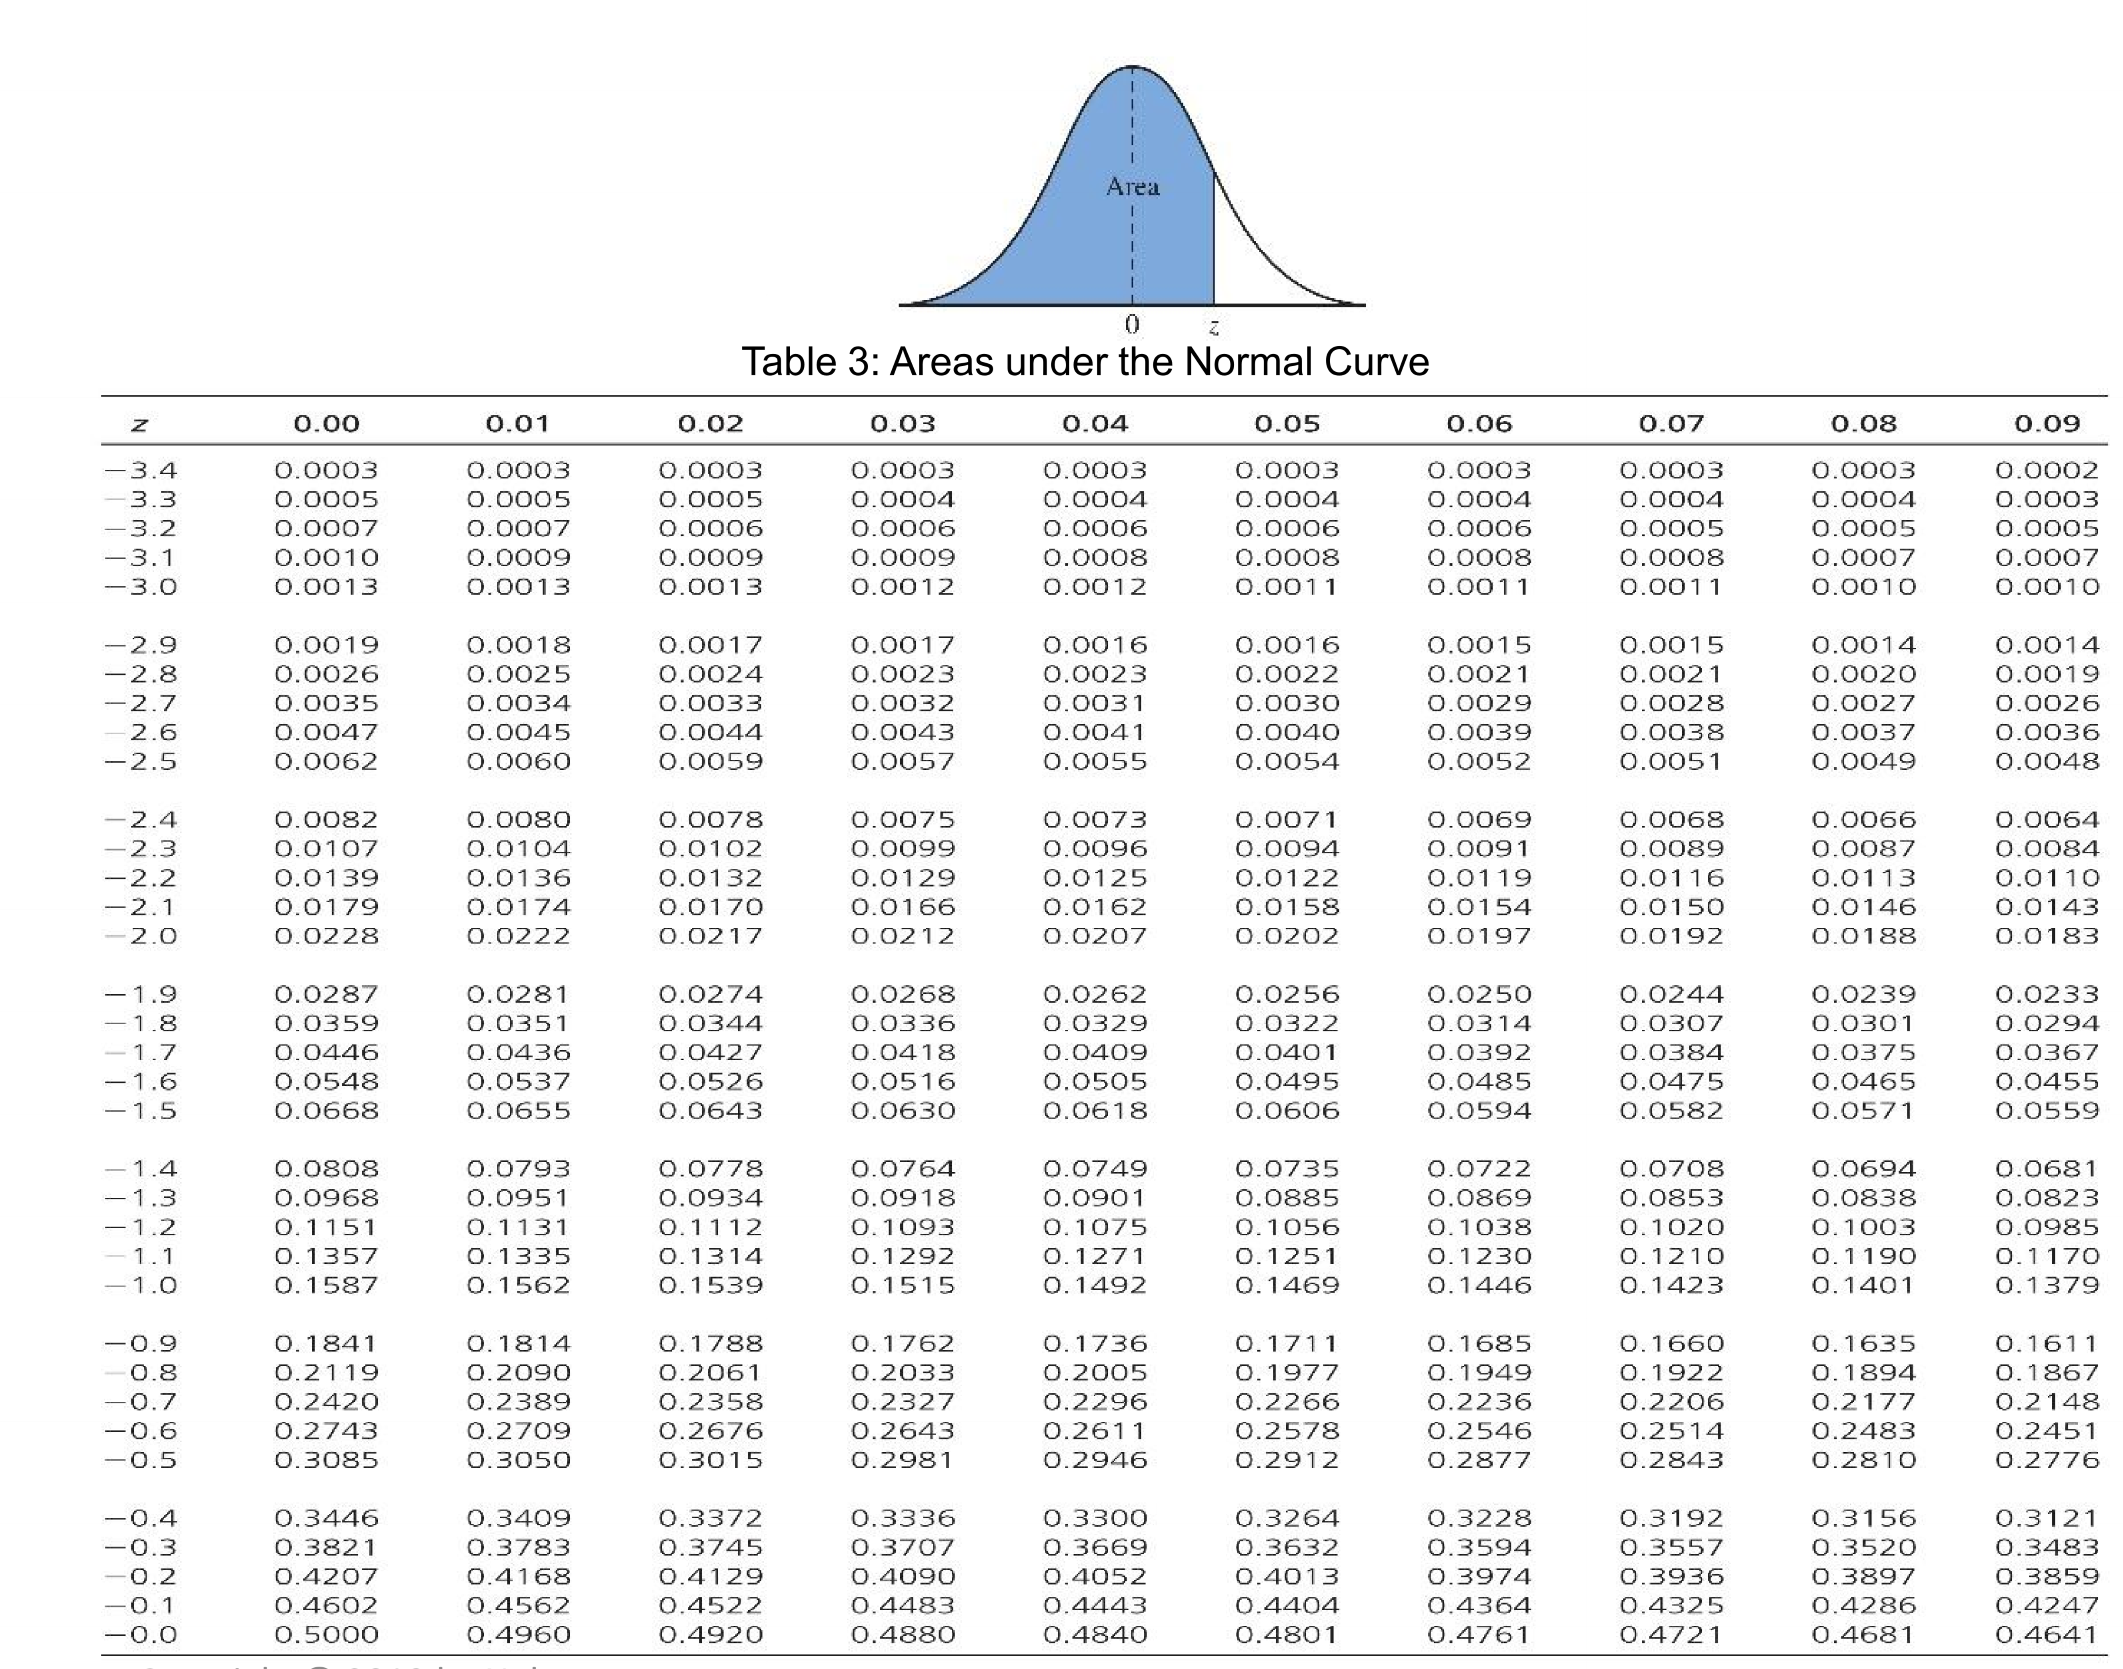
\includegraphics[width=0.85\textwidth]{appendix_images/Table3_1.PNG}
	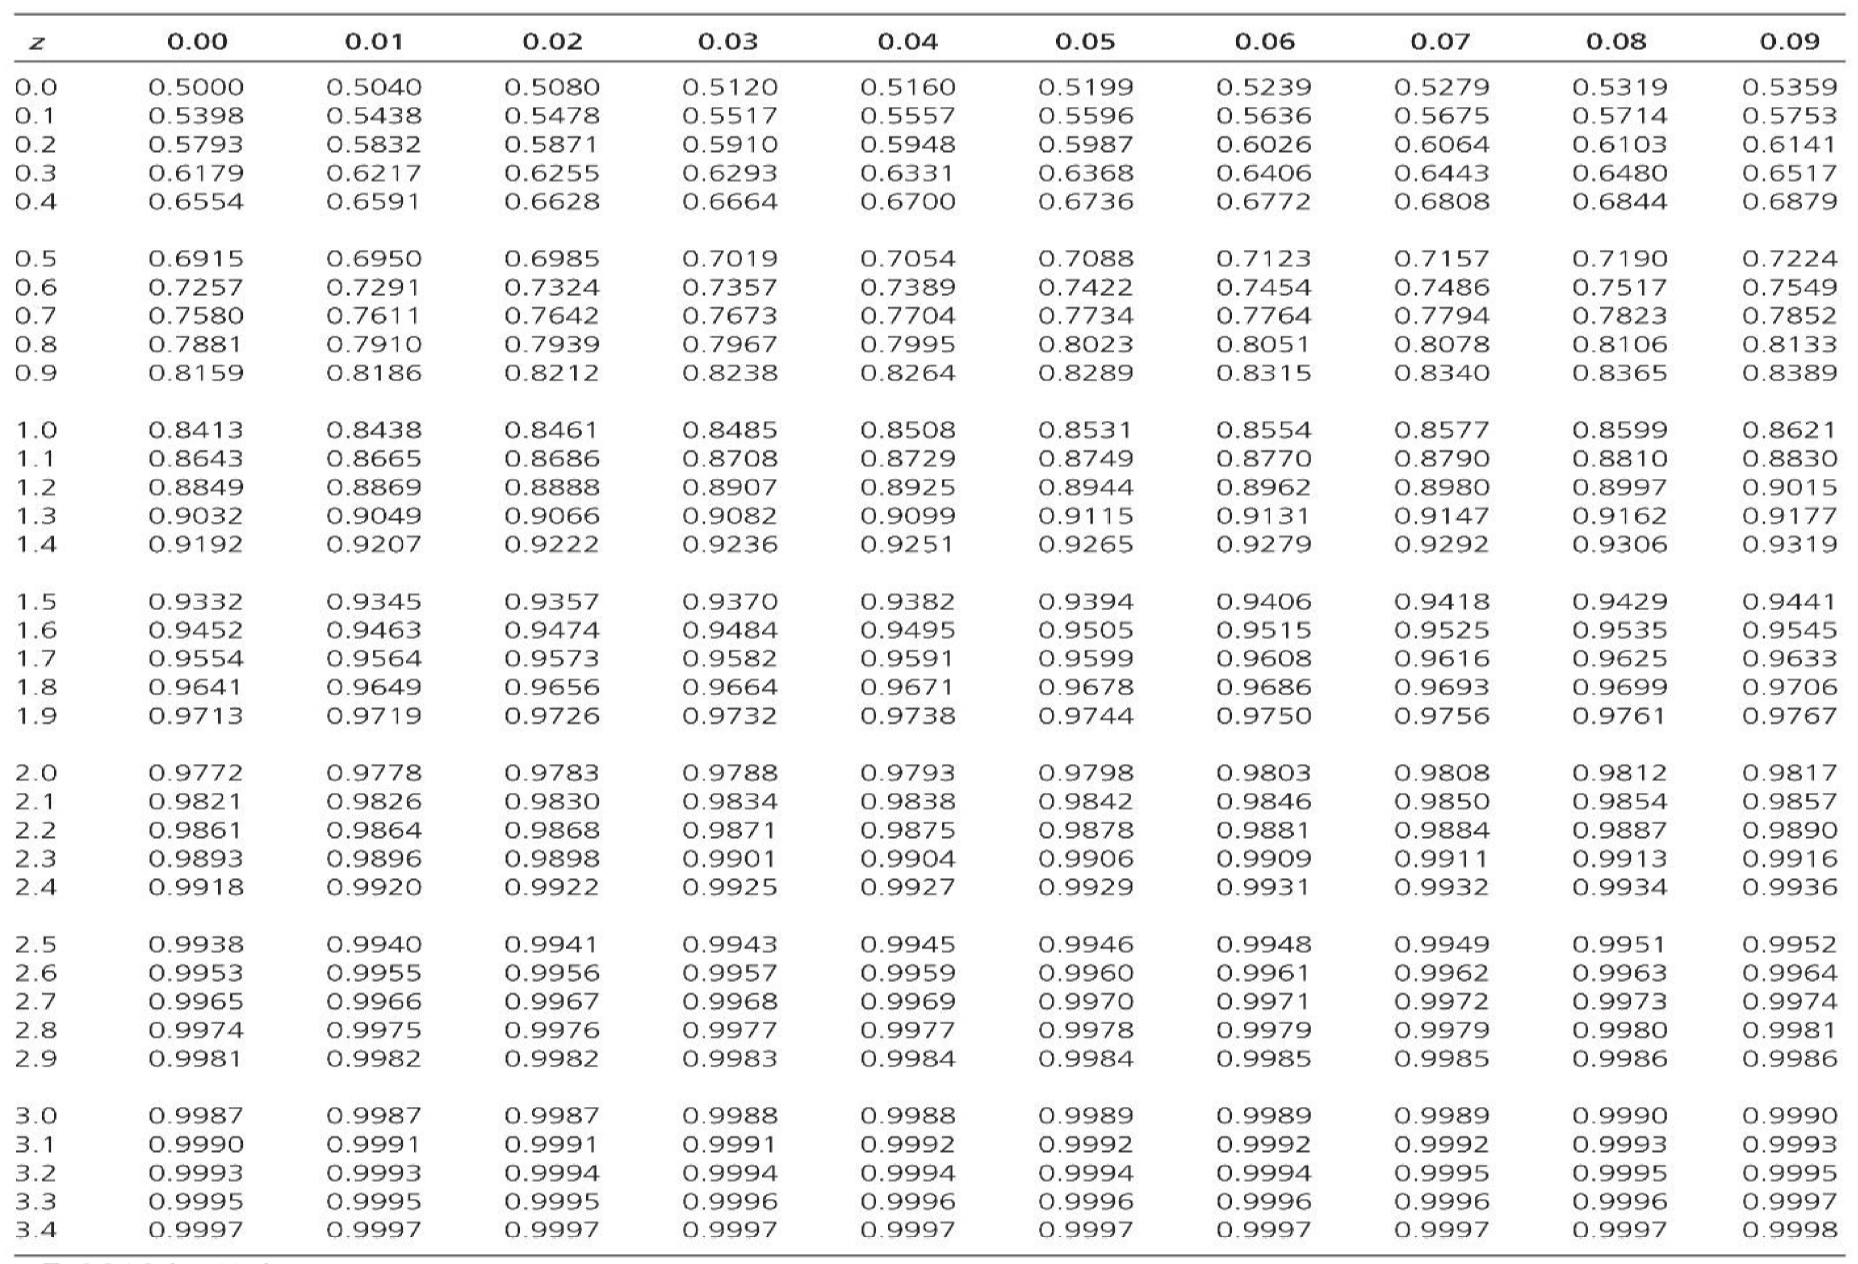
\includegraphics[width=0.80\textwidth]{appendix_images/Table3_2.PNG}
\end{center}


\end{document}